\section{調査}
\subsection{動画・画像の活用件数の推移}
図\ref{content_trend}は,動画及び画像の活用件数の含有率の年別推移である.
2016年までは,画像の活用は0.01\%未満であり,動画に関しては0件であった.
2017年以降,活用件数は急激に増加し,2021年には,動画~0.72\%,画像~5.93\%であった.
2017年以降に急激に増加した要因に関しては,調査中である.

\begin{figure}[t]
  \begin{center}
      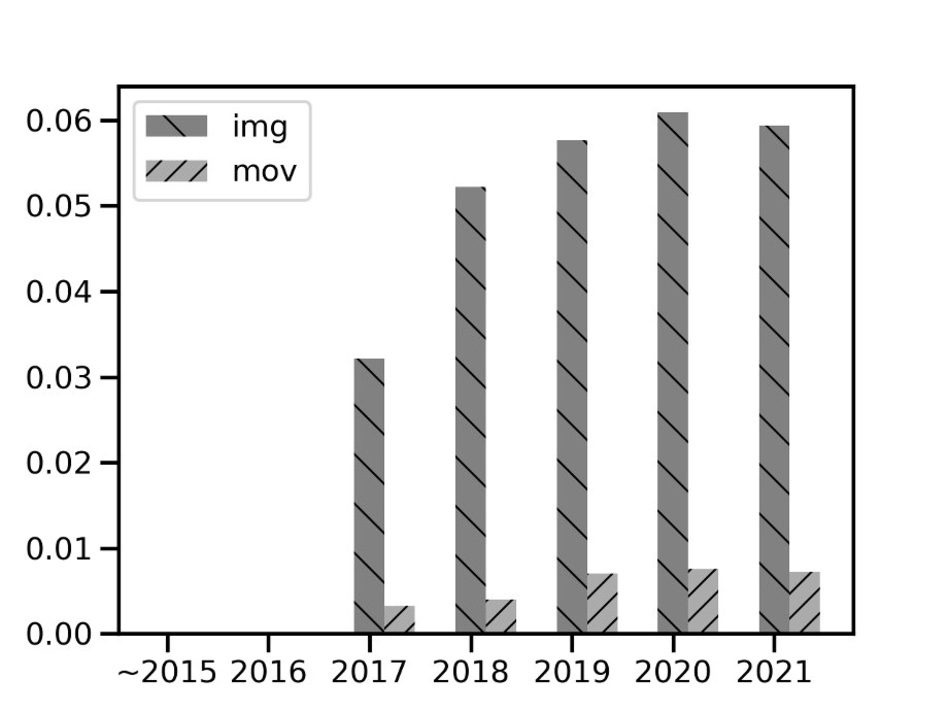
\includegraphics[scale=0.5]{./image/data_content_trends.pdf}
      \caption{動画・画像の含有率推移 \label{content_trend}}
  \end{center}
\end{figure}

\subsection{データの分析}

\begin{figure*}[t]
  \begin{center}
      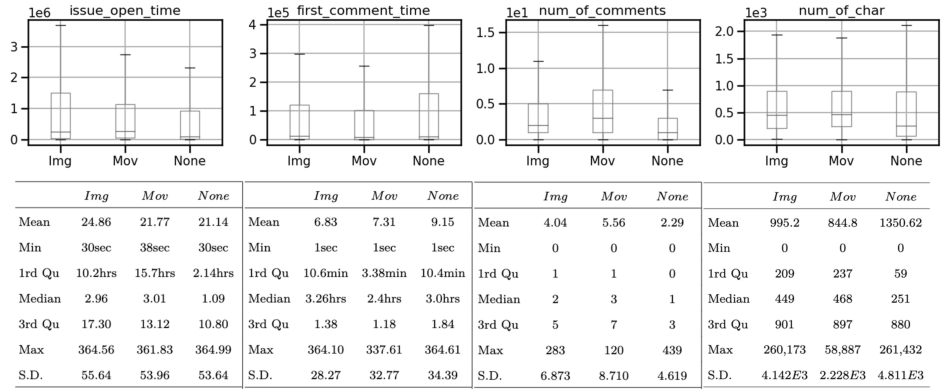
\includegraphics[scale=1.1]{./image/dataset_plot.pdf}
      \caption{Issue群ごとの調査項目の分布及び代表値 \label{dataset_plot}}
  \end{center}
\end{figure*}

図\ref{dataset_plot}は,データの特性値を箱ひげ図及び表で表現したものである.
ただし,図\ref{dataset_plot}の箱図の最大値は,$3rd~Qu + 1.5 * IQR$以下の最大値である.
($IQR$:四分位範囲)
\\
% この様な処理は,データの中央値付近を見やすくする為にしばしば用いられる.
\noindent{\bf{正規性について.}}
%図\ref{dataset_plot}では,$Issue\_open\_time$,$First\_comment\_time$及び$Num\_of\_char$の平均値が,
%四分位範囲内に収まっていないことから正規分布から逸脱している.
%$Num\_of\_comments$に関しては,正規分布しているような印象を受ける.
%実際,$Img$の平均値 = 4.04,標準偏差$S.D.$ = 6.873であり,これから$\pm~3S.D.$の上限値は24.66と算出できる.
%これから,最大値283は外れ値であるとも考えられる.しかし,
$Kolmogorov-Smirnov$検定の結果,すべての項目に対して,正規性は有意水準0.05で棄却された.
\\
\noindent{\bf{等分散性について.}}
$Leneve$検定の結果を表\ref{levene_result}に示す.
帰無仮説は「すべてのIssue群間を通して等分散」であり,有意水準は0.20とする.

\begin{table}[h]
  \begin{center}
  \caption{等分散性検定・結果}
  \begin{tabular}{l|c c} 
    \hline
     & 有意確率 & 平均分散比 \\ 
    \hline \hline
    $Issue\_open\_time$ & 0.378 & 1.050 \\
    $First\_comment\_time$ & 0.296 & 1.301 \\
    $Num\_of\_comments$ & 0.001 & 2.459 \\
    $Num\_of\_char$ & 0.073 & 3.156 \\
    \hline
  \end{tabular}
  \label{levene_result}
  \end{center}
\end{table}

$Num\_of\_comments$及び$Num\_of\_char$は,等分散性が有意水準0.20で棄却される.
$Issue\_open\_time$及び$First\_comment\_time$は,有意確率が有意水準以上であることと,
平均分散比が~1~\textasciitilde ~1.5~程度であることから,等分散性を仮定する.


\subsection{統計的検定}
本小節の目的は,群間の分布の差が統計的に有意であるかの検定である.
検定には,正規性及び等分散性を仮定しない$Steel-Dwass$法を用いる.
$Steel-Dwass$法による検定結果を表\ref{Steel-Dwass_result}に示す.
ただし,有意水準は0.05とする.

\begin{table}[t]
  \begin{center}
  \caption{調査項目ごとの多重比較の結果}
  \begin{tabular}{l r|r}
    \hline
    調査項目 & 対 & 有意確率 \\
    \hline \hline
    $Issue\_open\_time$ & & \\
     & \bf{$Img$~vs~$None$} & **~0.002 \\
     & \bf{$Mov$~vs~$None$} & **~0.021 \\
     & \bf{$Img$~vs~$~Mov$} & 0.381 \\
    \hline
    $First\_comment\_time$ & & \\
     & \bf{$Img$~vs~$None$} & 0.764 \\
     & \bf{$Mov$~vs~$None$} & 0.351 \\
     & \bf{$Img$~vs~$~Mov$} & 0.404 \\
    \hline
    $Num\_of\_comments$ & & \\
     & \bf{$Img$~vs~$None$} & *~0.001 \\
     & \bf{$Mov$~vs~$None$} & *~0.001 \\
     & \bf{$Img$~vs~$~Mov$} & 0.211 \\
    \hline
    $Num\_of\_char$ & & \\
     & \bf{$Img$~vs~$None$} & *~0.001 \\
     & \bf{$Mov$~vs~$None$} & *~0.001 \\
     & \bf{$Img$~vs~$~Mov$} & 0.599 \\
    \hline
  \end{tabular}\\
  \small
    *~ : 両側検定で有意 ~~~ ** : 片側検定で有意\\
  \label{Steel-Dwass_result}
  \end{center}
\end{table}

$Img$及び$Mov$は,$None$に比べて,$Issue\_open\_time$が有意に大きく,
$Num\_of\_comments$及び$Num\_of\_char$については分布に何らかの有意な差があると解釈できる.
一方で,$First\_comment\_time$においては,有意差は認められなかった.
また,$Img$と$Mov$の比較では,すべての項目で有意差は認められなかった.
有意差が認められなかった項目については,有意差の有無は判断を保留する.

\subsection{出現単語分析}
Issueのテキストに含まれる単語を\textbf{tf\_idf}値に変換し,同じIssue群に属すもの同士をマージした結果,\textbf{tf\_idf}値が大きい順に10個の結果を表\ref{tf-idf_result}に示す.
"at"や"it","the"などの単語を除外する為,
名詞,動詞及び疑問詞のみを対象とした. \\

\begin{table}[t]
  \begin{center}
  \caption{Issue群ごとの\textbf{tf\_idf}上位10単語}
  \begin{tabular}{r | c c c }
     & $Img$ & $Mov$ & $None$\\
    \hline \hline
    1 & image & when & dependabot\\
    2 & screenshot & dropdown & code\\
    3 & when & view & file\\
    4 & error & package & pullrequest\\
    5 & screen & issue & version\\
    6 & version & python & error\\
    7 & shot & height & use\\
    8 & file & react & lib\\
    9 & test & button & add\\
    10& code & text & commit\\
  \end{tabular}\\
  \label{tf-idf_result}
  \end{center}
\end{table}